%%%% DRAFT - SIMPLE TEXT %%%%%%

%% This is intended to provide examples of how to do such things as
%% include tables, figures, and program listings, and adjust layout,
%% etc. within TeX and LaTeX. It is in no way a substitute for the
%% many helpful resources which may be found online.  A few such
%% references are listed at the end of the main part of this document.

%% Lines (or parts of lines) such as these following percent sign '%'
%% are COMMENTS which do not appear in the output typeset document

%%%%%%% USEPACKAGE commands:

%% The \usepackage commands in the first section below load additional
%% packages in LaTeX to allow some extra commands, mostly for
%% convenience. Not all those here are needed in this document, but it
%% usually does no harm to include them, and many others are
%% available.  For example:

%% amssymb,amsmath:  These are part of the American Mathematical
%%                   Society distribution - extremely useful for
%%                   mathematical typesetting.

%% enumerate:  Governs enumerated list using \item

%% verbatim:   Allows text file to be included as it is - see \verbatiminput

%% ifpdf:      See note on Graphics below

%% For more information, see references cited at end of this doument
%% such as http://tobi.oetiker.ch/lshort/lshort.pdf

%%%%%% Note about including GRAPHICS FILES:

%% Some TeX implementations allow users to generate PDF output
%% directly while others produce DVI files (for example the commands
%% pdflatex or latex on Linux). These are interchangeable in most
%% respects but differ in the graphics formats which they expect when
%% including figures.  In particular, implementations producing PDF
%% files generally need PDF graphics files, while implementations
%% producing DVI files generally need PostScript files.  Discussion of
%% the relative merits is beyond the intended scope of this document.

%% In some implementations, the implementation is clever enough to
%% choose the right graphics files. For others, a command \ifpdf
%% (enabled by \usepackage ifpdf) is available which can allow for
%% EITHER option, switching automatically to look for a named figure
%% in the correct format.  For most users this will not be needed as
%% they will just use one or other type of latex processing, and we
%% will not use this here.

%%%%%% PREAMBLE, AND START AND END:

%% The first few lines beginning \documentstyle are to set up some
%% optional preferences in place of the defaults

%% The main part of the document always begins with "\begin{document}"
%% and ends with "\end{document}".

\documentclass[11pt,a4paper]{article}

  \usepackage[hmargin={25mm,25mm},vmargin={25mm,25mm}]{geometry}

  \usepackage{verbatim, ifpdf}
  \usepackage{graphicx, color}

% \usepackage{amssymb, amsmath}
% \usepackage{enumerate}

% *********************************************************************
% The following lines should be ignored unless you know what you are
% doing, since the hyperref package is somewhat temperamental! 

  \IfFileExists{hyperref.sty}{%
    \ifpdf
      \usepackage[pdftex]{hyperref}
    \else
      \usepackage[dvips]{hyperref}
    \fi
    \definecolor{maroon}{RGB}{128,0,0}
    \hypersetup{pdfborder=0 0 0,colorlinks=true,plainpages=false,
                pageanchor=true,linkcolor=black,urlcolor=maroon}%
  }{%
    \providecommand{\url}[1]{\texttt{##1}}
    \providecommand{\href}[2]{##2\footnote{~See \texttt{##1}.}}%
  }

% End of hyperref setup.
% *********************************************************************

% The following optional parameters adjust paragraph spacing and
% indentation
  \setlength{\parskip}{1ex plus 0.5ex minus 0.2ex}
  \setlength{\parindent}{0pt}
  \addtolength{\skip\footins}{1.5 mm}

%%%%%  END OF PREAMBLE %%%%%%%%%%%%%%%%

%%%%%  THE MAIN TEXT STARTS HERE %%%%%%

\begin{document}


\begin{center}\LARGE\bf
  Comments on the Phylogeography Project
\end{center}

\section*{A Note on Using the Cluster}

My working directory in the Cluster was \textbf{/nfs/research1/goldman/kalkauskas/} and the files of the project are in \textbf{/nfs/research1/goldman/kalkauskas/Phylogeography/}.

I also worked initially to some extent in \textbf{/hps/research1/goldman/kalkauskas/} and in \textbf{/homes/kalkauskas/} but all of the important work was moved to \textbf{/nfs/research1/goldman/kalkauskas/}.

Any computationally intensive tasks on the Cluster (such as running simulations or installing Anaconda) should be submitted as jobs. To read about it please refer to the link bellow:
\url{https://tsc.ebi.ac.uk/article/systems-infrastructure/technical-wiki}
\section*{Git Repository}

The git repository is here: \url{https://github.com/AntanasKal/Phylogeography}

\begin{verbatim}
git clone https://github.com/AntanasKal/Phylogeography.git
\end{verbatim}

\section*{Installing Anaconda}

Anaconda has to be installed. I do not remember how exactly I did that, but here are notes by Claudia on installing Anaconda:

\begin{verbatim}
wget https://repo.continuum.io/archive/Anaconda3-5.1.0-Linux-x86_64.sh
#see https://www.anaconda.com/download/#linux
bash Anaconda3-5.1.0-Linux-x86_64.sh
#add to .bashrc, then log out and back in
\end{verbatim}

\section*{Python libraries}

Python libraries not included in Anaconda package that had to be installed:

\begin{itemize}
\item dendropy
\item ercs
\item discsim
\item pymc3 (only needed to analyse output data, namely find HPD interval)
\end{itemize}

\url{https://dendropy.org/}

\url{https://github.com/jeromekelleher/discsim}

\url{https://pypi.org/project/ercs/}

\section*{Installing BEAST}

In the cluster I installed BEAST so that I could run it from command line (by adding PATH variable in \textbf{./bashrc}) following this tutorial: \url{https://beast.community/install_on_unix}.

Then BEAST could be run with Python by:

\begin{verbatim}
beast -overwrite -seed 123456795 "beast_xml_file.xml"
\end{verbatim}

But it might be easier to run BEAST from jar file. Just copy the \textbf{beast.jar} to a convenient directory and run:

\begin{verbatim}
java -jar beast.jar -overwrite -seed 123456795 "beast_xml_file.xml"
\end{verbatim}

If needed, BEAGLE can also be installed, but I did not use it.

Note that Python code might need to be changed in order to run 


\section*{Building PHYREX}
To build PHYREX binary from source use the following code:
\begin{verbatim}
git clone https://github.com/stephaneguindon/phyml.git
cd phyml
sh ./autogen.sh
./configure --enable-phyrex
make clean
make
\end{verbatim}

Afterwards in \textbf{src/} folder there will be \textbf{phyrex} binary file which can be placed in different different directory and it can be run by:

\begin{verbatim}
./phyrex --xml=file_name.xml
\end{verbatim}

\clearpage

\section*{How to Use the Code}



\subsection*{simulation.py}


Script \textbf{simulation.py} is the main script of the code. It simulates the phylogeny of a tree and Brownian motion along it, subsamples the tree in 4 scenarios, generates the needed files for BEAST and launches BEAST on these 4 subsampling scenarios.

\begin{verbatim}
python simulation.py 
\end{verbatim}

Some of the parameters of the program:

\begin{itemize}
\item \textbf{-N}: number of simulations in sequence in one run.
\item \textbf{-jobi}: index of a job. It is needed if we want to do a number of simulations in parallel and keep the track of files. So if \textbf{jobi} is $j$ and \textbf{N} is $n$, the simulations will be done and files will be generated for indices
$$nj, \ nj+1, \ ... , \ n(j+1) - 1$$ 

Usually I set \textbf{N} to 1 and iterate \textbf{jobi} from 0 to 99, so that 100 simulations would be done.


\item \textbf{-dims}: number of dimensions (1 or 2) for which the random walk is generated (default: 2). \textbf{Note:} for 1 dimension some parts of code might not work so they need to be commented out. These are some parts of the code that generate some less important output.

\item \textbf{-treetype}: type of tree generated.

nuc - nonultrametric coalescent

uc - ultrametric coalescent

bd - birth-death tree

yule - Yule tree

(default is "yule")
\item \textbf{-mcmc}: MCMC chain length for BEAST (default is 5000)

\item \textbf{-{}-linux}: whether the program is run on Cluster (different console commands are used the for executing BEAST).

\item \textbf{-ntips}: number of tips for ultrametric coalecent, birth-death and Yule trees (default 100)

\item \textbf{-ntipspp}: number of tips per period for nonultrametric coalescent trees (default 20).

\item \textbf{-nps}: number of periods for nonultrametric coalescent trees (default 25).

\item \textbf{-{}-c\_beast}: whether the program should generate input files (not output) for corrected BEAST.


\end{itemize}

Other parameters could be seen by:

\begin{verbatim}
python simulation.py -h
\end{verbatim}


Shell script \textbf{run\_beast.sh} runs 100 simulations on Cluster in parallel.
\begin{verbatim}
for i in $(seq 0 99)
do bsub -o console_output/out_"$i".txt -e console_output/err_"$i".txt\
python simulation.py -jobi "$i" -N 1 -dims 2\
-treetype yule -ntips 2000 --linux -mcmc 10000 --c_beast
done
\end{verbatim}


These simulation should take not much longer than 10 minutes to run. To run corrected BEAST the script \textbf{launch\_corrected\_beast.py} is needed. It takes the files previously generated by \textbf{simulation.py} and runs BEAST on them. These runs could take about 10 hours. The script has these parameters:

\begin{itemize}
\item \textbf{-sample\_index}: index of the sampling scenario (usually from 1 to 4)
\item \textbf{-i}: index of the simulation (usually from 0 to 99)
\end{itemize}

The shell script \textbf{run\_c\_beast.sh} executes \textbf{launch\_corrected\_beast.py} on all the files generated.
\begin{verbatim}
for i in $(seq 0 99)
do bgadd -L 10 /c_beast/sim"$i"
bsub -g /c_beast/sim"$i" -o console_output/c_beast_out1_"$i".txt\
-e console_output/c_beast_err1_"$i".txt\ 
python launch_corrected_beast.py -index $i -sample_index 1
bsub -g /c_beast/sim"$i" -o console_output/c_beast_out2_"$i".txt\
-e console_output/c_beast_err2_"$i".txt\
python launch_corrected_beast.py -index $i -sample_index 2
bsub -g /c_beast/sim"$i" -o console_output/c_beast_out3_"$i".txt\
-e console_output/c_beast_err3_"$i".txt\
python launch_corrected_beast.py -index $i -sample_index 3
bsub -g /c_beast/sim"$i" -o console_output/c_beast_out4_"$i".txt\
-e console_output/c_beast_err4_"$i".txt\
python launch_corrected_beast.py -index $i -sample_index 4
done
\end{verbatim}

\subsection*{treegenerator.py}

Script \textbf{treegenerator.py} generates the trees in various scenarios.
\begin{itemize}
\item \textbf{treegenerator.generate\_ultrametric\_coalescent\_tree(num\_tips, lamb)}: returns ultrametric coalescent tree with \textbf{num\_tips} of leaves and coalescent rate \textbf{lamb}.

\item \textbf{treegenerator.generate\_yule\_tree(num\_tips, br)}: returns a Yule tree with \textbf{num\_tips} leaves and birthrate \textbf{br}.

\item \textbf{treegenerator.generate\_nonultrametric\_coalescent\_tree(num\_tips\_per\_period, num\_periods, period\_length, lamb)}: returns nonultrametric coalescent tree with \textbf{num\_periods} of periods, \textbf{num\_tips\_per\_period} of tips per period, \textbf{period\_length} of time between periods and coalescent rate \textbf{lamb}

\item \textbf{treegenerator.generate\_birthdeath\_tree(num\_extinct, br, dr)}: returns a subtree of a birth-death with leaves being the first \textbf{num\_extinct} extinct nodes. Birthrate is \textbf{br} and deathrate is \textbf{dr}.
\end{itemize}

Other functions in the script that are useful:

\begin{itemize}
\item \textbf{treegenerator.simulate\_brownian(t, sigma, dimension)}: simulates Brownian motion along the tree \textbf{t} for $\sigma$ = \textbf{sigma} and returns the tree with every node having attributes \textbf{X} (and \textbf{Y} if \textbf{dimension} is 2).
\item \textbf{treegenerator.calculate\_times(t)}: calculates times of each node (seed node has time 0) and returns the tree with each node having \textbf{time} attribute.

\end{itemize}


\subsection*{sampling.py}

Script \textbf{sampling.py} is used to sample the tree according to different scenarios. The 4 ones that were mainly used are here:

\begin{itemize}
\item \textbf{sampling.sample\_unbiased(tree, dimension=2, sample\_ratio=0.1)}: returns subtree of \textbf{tree} with \textbf{sample\_ratio} of tips taken uniformly at random.

\item \textbf{sampling.sample\_biased\_most\_central(t, dimension=2, sample\_ratio=0.1)}: returns the subtree with leaves that are closest to the centre.

\item \textbf{sampling.sample\_biased\_diagonal(tree, dimension=2, sample\_ratio=0.1)}: returns the subtree with leaves that are closest to the diagonal.

\item \textbf{sampling.sample\_biased\_extreme(tree, dimension=2, sample\_ratio=0.1)}: returns the tree with leaves that have the largest $x$ coordinate.
\end{itemize}

\subsection*{Running PHYREX}

Script \textbf{run\_phyrex.sh} runs PHYREX on the output files generated.

\begin{verbatim}
for i in $(seq 0 99)
do bgadd -L 10 /yule/phyrex"$i"
bsub -g /yule/phyrex"$i" -o console_output/phyrex_out1_"$i".txt\
-e console_output/phyrex_err1_"$i".txt\
./phyrex --xml=output/phyrex/sampled1/phyrex_input/phyrex"$i".xml
bsub -g /yule/phyrex"$i" -o console_output/phyrex_out2_"$i".txt\
-e console_output/phyrex_err2_"$i".txt\
./phyrex --xml=output/phyrex/sampled2/phyrex_input/phyrex"$i".xml
bsub -g /yule/phyrex"$i" -o console_output/phyrex_out3_"$i".txt\
-e console_output/phyrex_err3_"$i".txt\
./phyrex --xml=output/phyrex/sampled3/phyrex_input/phyrex"$i".xml
bsub -g /yule/phyrex"$i" -o console_output/phyrex_out4_"$i".txt\
-e console_output/phyrex_err4_"$i".txt\
./phyrex --xml=output/phyrex/sampled4/phyrex_input/phyrex"$i".xml
done
\end{verbatim}

\subsection*{Other Scripts}
Scripts \textbf{beastxmlwriter.py} and \textbf{phyrexxmlwriter.py} are used for writing BEAST and PHYREX input files respectively.

\section*{Discsim Scripts}

If $\lambda$ is the rate of events is $\Lambda V$ model, $\mu$ is the death probability, $L$ is the diameter of torus and $r$ is the radius of sampling circle, then the rate at which sampling event occurs at given point is
$$\frac{\lambda \pi r^2}{L^2}$$
Given that a point is hit, the probability that it is displaced is $\mu$. Also the mean square distance of one displacement is the mean square distance between two points chosen uniformly at random in the disc and it is $r^2$ (can be computed by integrating $$\int_D \left(\int_D(x_1-x_2)^2+(y_1-y_2)^2\frac{1}{\pi r^2}dx_1dy_1\right)\frac{1}{\pi r^2}dx_2dy_2$$

$$=\int_D \left(\int_D (x_1^2+x_2^2-2x_1x_2+y_1^2-2y_1y_2+y_2^2)\frac{1}{\pi r^2}dx_1dy_1\right)\frac{1}{\pi r^2}dx_2dy_2$$

$$=\int_D \left(\int_D (x_1^2+x_2^2+y_1^2+y_2^2)\frac{1}{\pi r^2}dx_1dy_1\right)\frac{1}{\pi r^2}dx_2dy_2$$

$$=\int_0^{2\pi} \int_0^{r} \int_0^{2\pi} \int_0^r  (\rho_1^2+\rho_2^2)\frac{1}{\pi^2 r^4} \rho_1\rho_2d\theta_1 d\rho_1 d\theta_2 d\rho_2$$

$$= \frac{4}{r^4}\int_0^{r}  \int_0^r  (\rho_1^2+\rho_2^2) \rho_1\rho_2 d\rho_1  d\rho_2= \frac{4}{r^4}\int_0^{r}  \int_0^r  (\rho_1^2+\rho_2^2) \rho_1\rho_2 d\rho_1  d\rho_2$$

$$= \frac{4}{r^4}\int_0^{r}\left(  \frac{r^4}{4}\rho_2+\rho_2^3\frac{r^2}{2}  \right)d\rho_2= \frac{4}{r^4}\left(  \frac{r^6}{8}+\frac{r^6}{8}  \right)=r^2$$




 where $D$ is a disc of radius $r$ centred at 0 and observing that terms such as $2x_1x_2$ integrate to 0).

So over a unit time, mean square displacement of an individual is
$$\frac{\lambda \mu \pi r^2}{L^2}r^2=\frac{\lambda \mu \pi r^4}{L^2}$$

For Lemey model with diffusion matrix being identity, mean square displacement over a unit time is 2. 

So having set $\lambda$, $\mu$, $r$, in order to get $\Lambda V$ process to be similar to Brownian motion as with diffusion rate being identity matrix we need to set

$$\lambda=\frac{2L^2}{\mu \pi r^4}$$

I have added the code to check this in Jupyter notebook "Phylogeography Output Analysis".



\subsection*{discs.py}

This script runs a discsim simulation, generates BEAST and PHYREX files for that and runs BEAST.
Currently it is set up in such a way that simulations indexed 0-99 are sampled from a square having opposite corners at $(25,\ 25)$ and $(75,\ 75)$, and simulations indexed 100-199 are sampled from a square having opposite corner at $(45,\ 45)$ and $(55,\ 55)$. It outputs the obtained root in folder \textbf{output/root\_data/}.



Shell script \textbf{run\_discs.sh} runs the 200 simulations:

\begin{verbatim}
bgadd -L 200 /discs
for i in $(seq 0 200)
do bsub -g /discs -o console_output/out_"$i".txt -e\
console_output/err_"$i".txt python discs.py -jobi "$i" -N 1
done
\end{verbatim}

Shell script \textbf{run\_phyrex.sh} runs PHYREX on all the simulations:

\begin{verbatim}
bgadd -L 200 /LV_phyrex
for i in $(seq 0 199)
do bsub -g /LV_phyrex -o console_output/phyrex_out_"$i".txt\
-e console_output/phyrex_err_"$i".txt\
./phyrex --xml=output/phyrex/LV/phyrex_input/phyrex"$i".xml
done  
\end{verbatim}



\subsection*{Other scripts}

Script \textbf{newick.py} for converting directed trees outputted by discsim to newick trees.
I edited this script after taking it from here:

\url{https://github.com/tyjo/newick.py/blob/master/newick.py}

Scripts \textbf{treegenerator.py} and \textbf{beastxmlwriter.py} in the folder are just copies of these scripts from Phylogeography folder.

Script \textbf{disc\_phyrexxmlwriter.py} is edited script \textbf{phyrexxmlwriter.py} to write  PHYREX xml scripts in this case.


\section*{Output Folders}
Output is organised in this way: \textbf{output} folder has subfolders 
\textbf{beast}, \textbf{c\_beast}, \textbf{phyrex} which contain input and output files of BEAST, corrected BEAST and PHYREX. Each of these folders contains 4 folder for the results of 4 sampling scenarios. There are a few other folders, but they are not necessary.
The \textbf{.trees.txt} files take lots of space and only the root locations were important for us. Processed root locations are put into \textbf{root\_data/} folders and if I am downloading the data to my computer I usually delete the \textbf{.tree.txt} files by going to the folders containing them and executing this command:

\begin{verbatim}
find . -name "*.trees.txt" -type f -delete
\end{verbatim} 


Here is a rough scheme of the \textbf{output/} folder:
\begin{itemize}
\item \textbf{beast}
\begin{itemize}
\item \textbf{sampled1}
\begin{itemize}
\item \textbf{beast\_input}
\item \textbf{beast\_output}
\item \textbf{root\_data}
\end{itemize}
\item \textbf{sampled2}
\begin{itemize}
\item ...
\end{itemize}
\item \textbf{sampled3}
\begin{itemize}
\item ...
\end{itemize}
\item \textbf{sampled4}
\begin{itemize}
\item ...
\end{itemize}
\end{itemize}

\item \textbf{phyrex}
\begin{itemize}
\item \textbf{sampled1}
\begin{itemize}
\item \textbf{phyrex\_input}
\item \textbf{phyrex\_output}
\end{itemize}
\item ...

\end{itemize}

\item \textbf{c\_beast}
\begin{itemize}
\item ...
\end{itemize}





\end{itemize}

\clearpage


This is an example of a short document typeset using \LaTeX\ to show
some features such as the inclusion of
\begin{itemize}
\item tables,
\item figures, and
\item single and multi-line equations.
\end{itemize}

% In future a file \texttt{example.tex} may be made available for
% possible use as a template, with some features of this guide, and
% additional comments and details.

This document is in no way a substitute for the many helpful resources
which may be found online, of which a few suggestions are given at the
end of the main part of this document.

Note that although \LaTeX\ is well suited for mathematical
typesetting, it is absolutely acceptable to write reports using other
word-processing software (such as Microsoft Word or LibreOffice).
%
%, or to submit handwritten reports, or a combination.  For example, a
% mixture of typeset text and handwritten equations may be perfectly
% fine.
%
See \S\,2.3 of the \textsl{Introduction} to the \textsl{Computational
  Projects Manual} for general guidance.

\subsection{Finding a \LaTeX\ program}

If you decide to use a \LaTeX, or you wish to try it out, \LaTeX\ is
available on the University's \textsl{Managed Cluster Service}. If you
are going to use it extensively, then you will probably want to
install \LaTeX\ on your own personal computer. This can be done for
free, e.g.\ for recommendations and packages see
\begin{itemize}
\item \url{http://www.tug.org/begin.html\#install} and
\item \url{http://www.tug.org/interest.html\#free}
\end{itemize}
As a `front-end' (i.e.\ `clever editor'), Mac users will probably want
to use \href{http://pages.uoregon.edu/koch/texshop/}{{\TeX}Shop},
while for Windows and Linux users (and Mac users) there is,
\textit{inter alia}, \href{http://www.tug.org/texworks/}{{\TeX}works};
see the \textsl{Introduction} to the
\href{http://www.maths.cam.ac.uk/undergrad/catam/IB/}{Part~IB} or
\href{http://www.maths.cam.ac.uk/undergrad/catam/II/}{Part~II}
\textsl{Computational Project Manuals} for more details.

\subsection{Setting up the document}\label{setup}

At the start of your document you will need commands to set up the
style, font-size, and other personal preferences.  Many of these are
\textit{optional}, but the main body of text to be typeset must start
with
\begin{quote}
\verb|\begin{document}|
\end{quote}
and end with
\begin{quote}
\verb|\end{document}|
\end{quote}

%  In future, more details and explanatory comments may be found in
% \S\,\ref{extras} below, and in \texttt{example.tex}.

As indicated in the \textsl{Computational Projects Manual}, you are
requested to leave a space 5cm by 11cm for a label at the top right
hand corner of the front page of your project. The box at the start of
this page was produced by the lines:
\begin{quote}
\begin{verbatim}
\hfill\framebox{\parbox[t][5 true cm][c]{11 true cm}
{\hfil Space for project label}}
\end{verbatim}
\end{quote}

\subsection{Headings, sections and subsections}

It is sensible to include headings and to organise your write-ups into
sections, subsections and subsubsections, e.g.\ so that your answer to
each question has a heading. For instance the document title was
produced by
\begin{quote}
\begin{verbatim}
\begin{center}\LARGE\bf
  A Brief \LaTeX\ Guide for CATAM
\end{center}
\end{verbatim}
\end{quote}
where the \verb!\! after the \verb!\LaTeX! command is necessary to
generate a space (you might like to experiment to see the effect of
omitting the \verb!\!).

\LaTeX\ has specific commands to generate sections, subsections,
subsubsections, etc. Moreover, it is possible to get \LaTeX\ to
number these automatically (the default). For instance,
\begin{itemize}

\item the first section heading in this document was produced by a
  line
\begin{quote}
\verb|\section{This document}|
\end{quote}

\item and, similarly, this subsection heading was produced by
\begin{quote}
\verb$\subsection{Headings, sections and subsections}$
\end{quote}
\end{itemize}

In order to omit the numbering, append \verb|`*'| to the command,
e.g.\ \verb|\section*{This document)|.

\subsection{Numbering and labels}

Objects such as figures, tables, equations, sections, and page numbers
can be referred to using \textit{labels}; the labels will be replaced
with the correct reference when typeset by \LaTeX.  For example, we
might wish to refer to a (sub)section by number, or to a program
listing by page number (e.g.\ page \pageref{question:2:program} in
this document), before knowing either what the section numbers is, or
on which page the program will occur in the final typeset document.

Numbered [sub-]sections are \textit{labelled} by adding a \verb!\label!
command after the [sub-]section name. For example, we can refer to
\S\,\ref{proglist} below, because the subsection heading is followed
by a label thus:
\begin{quote}
\begin{verbatim}
\subsection{Program listings and page number references}\label{proglist}
\end{verbatim}
\end{quote}
so allowing us to refer to the label \verb|proglist| from elsewhere in
the text by using, say, the reference `\verb|\S\,\ref{proglist}|'.

\subsection{Mathematical expressions}

Mathematical expressions such as $2x+5-3\sin x=0$ can be included
in-line by putting \$ signs around the expression to tell \LaTeX\ to
treat it as mathematics (where the upright `sin' is produced within
the \$ signs by using the command \verb|\sin|; similarly for `cos',
etc.).

It is also possible to produce `displayed' equations.  The equation
\begin{equation}
  |f^{\prime}(x_*)| \equiv \left|\frac{3\cos{x_*}+k}{2+k}\right| > 1 \,.
  \label{picard3}
\end{equation}
is produced using
\begin{quote}
\begin{verbatim}
\begin{equation}
  |f^{\prime}(x_*)| \equiv \left|\frac{3\cos{x_*}+k}{2+k}\right| > 1 \,.
  \label{picard3}
\end{equation}
\end{verbatim}
\end{quote}
The equation is numbered automatically, and has again been associated
with a label in order to refer to it by number elsewhere in the text;
thus the \LaTeX
\begin{quote}
  \verb| `see equation (\ref{picard3})'|
\end{quote}
produces `see equation (\ref{picard3})'.

Moreover,
\begin{itemize}
\item if the equations are subsequently re-ordered then, after a
  couple of invocations, \LaTeX\ will successfully automatically
  correct the references;
\item this use of labels also works for figures, tables, etc.\ (see
  below);
\item if you do not wish to number your equation[s],
  \begin{itemize}
  \item[$\circ$] either append a `\verb|*|' to \verb|equation| in
    \verb|\begin{equation} ... \end{equation}|,
  \item[$\circ$] or replace \verb|\begin{equation} ... \end{equation}| with
    \verb|\[ ... \]|.
  \end{itemize}
\end{itemize}

Sometimes an equation will not fit on a single line, or there are
multiple lines in an expression. \LaTeX\ almost always has a solution
to any typesetting problem. For instance. here is a more complicated
example of a single numbered equation split over multiple lines:
\begin{eqnarray}
x_N &=& x_{N-1} - \frac{F(x_{N-1})}{F'(x_{N-1})} \nonumber\\
    &=& x_* + \frac{F^{\prime\prime}\left(x_*\right)}
                   {2 F^{\prime}\left(x_*\right)}
              \left(x_{N-1}-x_*\right)^2 + \dots \,.
\end{eqnarray}
This was produced by
\begin{quote}
\begin{verbatim}
\begin{eqnarray}
x_N &=& x_{N-1} - \frac{F(x_{N-1})}{F'(x_{N-1})} \nonumber\\
    &=& x_* + \frac{F^{\prime\prime}\left(x_*\right)}
                   {2 F^{\prime}\left(x_*\right)}
              \left(x_{N-1}-x_*\right)^2 + \dots \,.
\end{eqnarray}
\end{verbatim}
\end{quote}
Here, the \verb|&| signs are used to align the equations -- in this
case at the equality signs. We also note that
\begin{itemize}
\item each line apart from the last must end with a `new line' symbol
  \verb|\\|;
\item the \verb|\nonumber| command can be used to tell \LaTeX\ not to
  number that line.
\end{itemize}

\subsection{Itemized lists}

This document has a number of itemized lists. For instance
\begin{quote}
\begin{verbatim}
\begin{itemize}
\item first item;
\item second item;
  \begin{itemize}
  \item[$\circ$] second item, first sub-item;
  \item[$\circ$] second item, second sub-item.
  \end{itemize}
\end{itemize}
\end{verbatim}
\end{quote}
produces
\begin{itemize}
\item first item;
\item second item;
  \begin{itemize}
  \item[$\circ$] second item, first sub-item;
  \item[$\circ$] second item, second sub-item.
  \end{itemize}
\end{itemize}
It is also possible to generate numbered lists; e.g.
\begin{quote}
\begin{verbatim}
\begin{enumerate}
   \item This is the first line.
   \item This is the second.
   \item Here's the third.
\end{enumerate}
\end{verbatim}
\end{quote}
produces
\begin{enumerate}
\item This is the first line.
\item This is the second.
\item Here's the third.
\end{enumerate}

\subsection{Example of a figure}

\LaTeX\ has many ways of inserting graphs. In what follows we assume
that the source file for the graph is in a sub-directory
\texttt{Plots}, and that the source file is called
\begin{itemize}
\item \texttt{Figure-1.pdf} if the graph is in PDF form;
\item \texttt{Figure-1.eps} (or \texttt{Figure-1.ps}) if the graph is in
  PostScript form.
\end{itemize}
If you are working with the \texttt{pdflatex} command on Linux (or
with its equivalents on Windows/Mac), then a graph in PDF form may be
preferable, although some modern versions of the \texttt{pdflatex}, or
its equivalents, command also accept graphs in PostScript form. If you
are working with the \texttt{latex} command, or its equivalents, then
the graph should not be in PDF form but in, say, PostScript form instead.

The following \LaTeX\ source \textsl{should} work with both the
\texttt{pdflatex} and \texttt{latex} commands on Linux, or with its
equivalents on Windows/Mac, and should insert the graph somewhere
\textsl{near} here!

% Also see the comments on including graphics in preamble.

\begin{quote}
\begin{verbatim}
\begin{figure}[ht]\centering\label{q3fig1}
  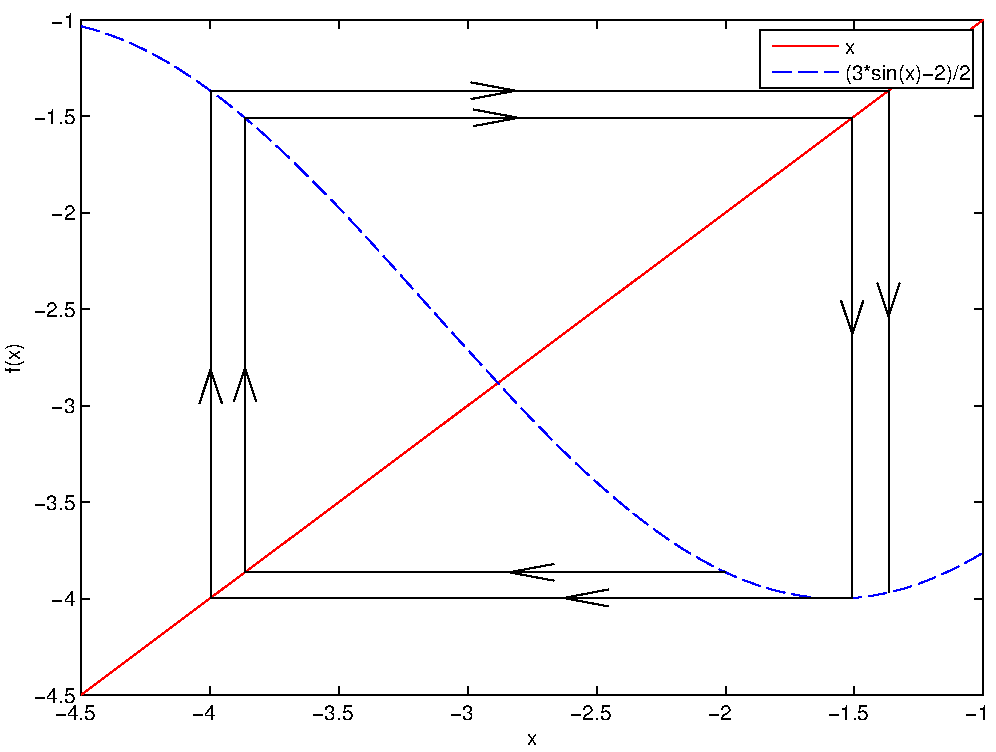
\includegraphics[height=78mm,angle=0]{Plots/Figure-1}
  \caption{A caption can go here. Figures can be numbered automatically.}
\end{figure}
\end{verbatim}
\end{quote}
\begin{figure}[ht]\centering\label{q3fig1}
  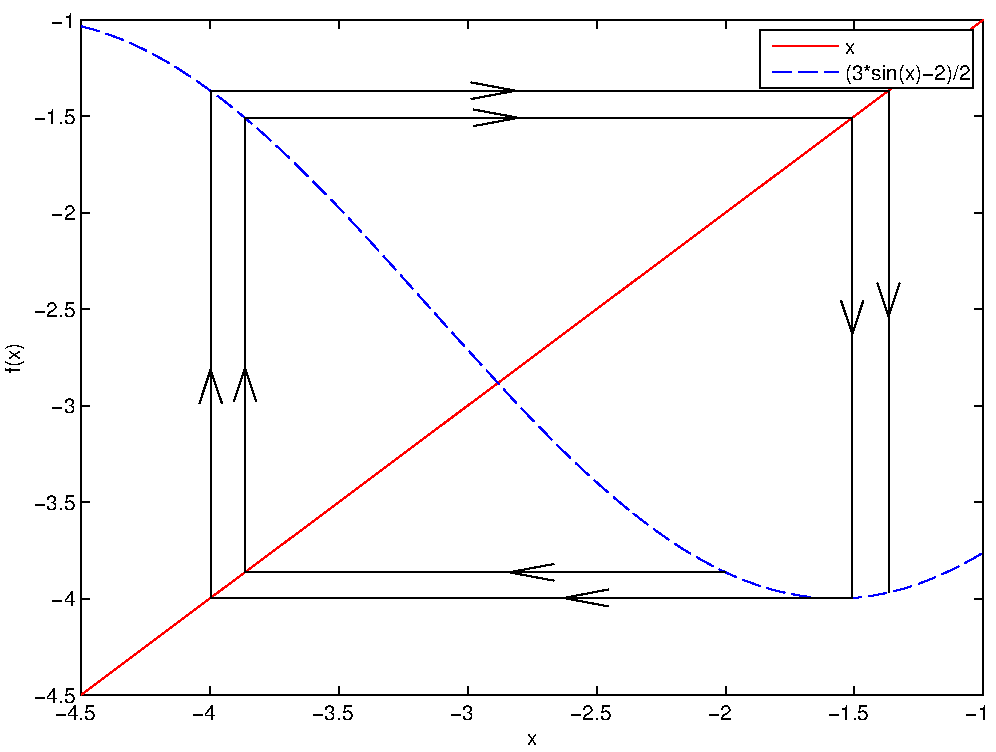
\includegraphics[height=78mm,angle=0]{Plots/Figure-1}
  \caption{A caption can go here. Figures are numbered automatically.}
\end{figure}
\textsl{Remarks}
\begin{itemize}
\item Figures `float', i.e.\ they are included when and where there is
  space; the \texttt{[ht]} specification means include the figure
  `\underline{\bf h}ere' or at the `\underline{\bf t}op of a page'.
\item Most modern versions of \LaTeX\ will append \texttt{.pdf} or
  \texttt{.eps} (or \texttt{.ps}) as appropriate to \texttt{Figure-1};
  if your version does not do this then you will need to add the
  suffix explicitly by editing the \verb|\includegraphics| line to
  refer to, say, \texttt{Plots/Figure-1.pdf}.
\item Many \texttt{latex} commands that produce DVI output will accept many
  different graphics formats in addition to PostScript (again you may
  have to edit the \verb|\includegraphics| line).
\end{itemize}

% In future more information on including graphics may be given in the
% accompanying template file.

\subsection{Example of a table}

You may have the need to present the output of calculations in a
table. The following commands produce the table which follows:
\begin{quote}
\begin{verbatim}
\begin{table}[ht]\centering\label{k=16:x=-2}
\caption{The table caption can go here.}\medskip\small
\begin{tabular}{ccccc}
 $N$ & $x_N$ & $\epsilon_N$ & $\epsilon_N/\epsilon_{N-1}$ &
 $f'(x_N)$\\[1mm]
   0 & -2.0000000 &  8.832369e-01 \\
   1 & -2.2071051 &  6.761317e-01 &  0.7655158 &  0.7898504 \\
   2 & -2.3736981 &  5.095388e-01 &  0.7536087 &  0.7689931 \\
&&&&\\[-4mm]
\vdots & \vdots & \vdots & \vdots & \vdots \\[ 2mm]
  32 & -2.8831971 &  3.981016e-05 &  0.7277548 &  0.7277554 \\
  33 & -2.8832079 &  2.897202e-05 &  0.7277545 &  0.7277549 \\
  34 & -2.8832158 &  2.108451e-05 &  0.7277543 &  0.7277546 \\
\end{tabular}
\end{table}
\end{verbatim}
\end{quote}
\begin{table}[ht]\centering\label{k=16:x=-2}
\caption{The table caption can go here.}\medskip\small
\begin{tabular}{ccccc}
 $N$ & $x_N$ & $\epsilon_N$ & $\epsilon_N/\epsilon_{N-1}$ &
 $f'(x_N)$\\[1mm]
   0 & -2.0000000 &  8.832369e-01 \\
   1 & -2.2071051 &  6.761317e-01 &  0.7655158 &  0.7898504 \\
   2 & -2.3736981 &  5.095388e-01 &  0.7536087 &  0.7689931 \\
&&&&\\[-4mm]
\vdots & \vdots & \vdots & \vdots & \vdots \\[ 2mm]
  32 & -2.8831971 &  3.981016e-05 &  0.7277548 &  0.7277554 \\
  33 & -2.8832079 &  2.897202e-05 &  0.7277545 &  0.7277549 \\
  34 & -2.8832158 &  2.108451e-05 &  0.7277543 &  0.7277546 \\
\end{tabular}
\end{table}
\begin{itemize}
\item As in the case of a \texttt{figure}, by using the \texttt{[ht]}
  specification, \LaTeX\ will try to place the table near to where it
  occurs in the source file, or failing that at the top of page.
\item The command \verb|\begin{tabular}{ccccc}| tells \LaTeX\ that
  there are 5 columns and the entries are to be \underline{\bf c}entred.
\item Column entries are separated by ampersand \texttt{\&}, and lines
  are terminated using \verb|\\|.
\end{itemize}

\subsection{Program listings and page number references}\label{proglist}

Program listings must be included at the end of your CATAM
reports. These \textsl{either} can be included separately, \textit{or}
can be included via your \LaTeX\ code. As an example we have included
a program from a file called \texttt{question2.m} (located in the
sub-directory \texttt{MATLAB}) at the end of this
brief guide, on page~\pageref{question:2:program}.  The \LaTeX\ code
to do this is as follows:
\begin{quote}
\begin{verbatim}
\begin{center}\label{question:2:program}
   Program \texttt{program-2.m} for Question 2
\end{center}
{\small \verbatiminput{MATLAB/program-2.m}}
\end{verbatim}
\end{quote}
\begin{itemize}
\item The line \verb|\label{question:2:program}| labels the page so
  that it can be referred to elsewhere in the text, say by
  \verb|`see the code on page \pageref{question:2:program}'| in which
  the label will be replaced automatically with the correct number,
  e.g.\ `see the code on page~\pageref{question:2:program}'.
\end{itemize}

% \subsection{Setting up the environment and extra commands}\label{extras}

% As mentioned in section (\ref{setup}) above, the document will start
% with optional commands.

\subsection{Some \LaTeX\ references}

Beginners, as well as more advanced users, may find some of the
following references helpful (all working at time of writing):
\begin{itemize}\small

% Encode ~ as \%7E and _ as \%5F for when hyperref is not available. ~
% is always are problem for LaTeX, and _ (or \_) will not cut and
% paste from acroread.

\item \url{http://physics.nyu.edu/\%7Ephyslab/Lab\%5FMain/Latexguide.pdf}
\item \url{http://www.cs.princeton.edu/courses/archive/spr10/cos433/Latex/latex-guide.pdf}
\item \url{http://www.maths.tcd.ie/\%7Edwilkins/LaTeXPrimer/}
\item \url{http://tobi.oetiker.ch/lshort/lshort.pdf}
\item \url{http://www.maths.adelaide.edu.au/anthony.roberts/LaTeX/index.php}
\item \url{http://en.wikibooks.org/wiki/LaTeX/}
\end{itemize}

% Here we begin a program listing, with input from a separate file.
% We use \clearpage rather than \newpage to clear floats.

\clearpage

\end{document}
